\subsection{Đề 05}
\caulc
\Opensolutionfile{ans}[ans/ans-CTST-0-OTGK1-De05-LC]
%%%Câu 1
\begin{ex}%[0D1N1-3]
	Cho mệnh đề $A\colon$\lq\lq $\forall x\in\mathbb{R}\colon x^2+1>0$ \rq\rq. Trong các mệnh đề sau, mệnh đề nào là phủ định của mệnh đề $A$?
	\choice
	{$\overline{A}\colon$\lq\lq$\exists x\in \mathbb{R}\colon x^2+1>0$ \rq\rq}
	{$\overline{A}\colon$\lq\lq$\forall x\in \mathbb{R}\colon x^2+1 \leq 0$ \rq\rq}
	{$\overline{A}\colon$\lq\lq$\forall x\in \mathbb{R}\colon x^2+1 \neq 0$ \rq\rq}
	{\True $\overline{A}\colon $\lq\lq$\exists x\in \mathbb{R}\colon x^2+1 \le 0$ \rq\rq}
	\loigiai{
		Mệnh đề phủ định $\overline{A}\colon$\lq\lq$\exists x\in \mathbb{R}\colon x^2+1\le 0$\rq\rq.	
	}
\end{ex}
%%%Câu 2
\begin{ex}%[0D1N2-1]
	Cho tập hợp $A=\{x\in\mathbb{Z}\big|-3<x\le 4\}$. Khẳng định nào sau đây đúng?
	\choice
	{\True $A=\{-2;-1;0;1;2;3;4\}$}
	{$A=(-3;4]$}
	{$A=\{-2;-1;0;1;2;3\}$}
	{$A=\{-3;-2;-1;0;1;2;3;4\}$}
	\loigiai{
		Ta có tập hợp $A=\{-2;-1;0;1;2;3;4\}$. 	
	}
\end{ex}
%%%Câu 3
\begin{ex}%[0D1N3-2]
	Cho hai tập hợp $A=(1;5]$; $B=(2;7]$. Tập hợp $A\setminus B$ là
	\choice
	{\True $(1;2]$}
	{$(2;5)$}
	{$(-1;7]$}
	{$(-1;2)$}
	\loigiai{
		Ta có $A\setminus B=(1;2]$. 	
	}
\end{ex}
%%%Câu 4
\begin{ex}%[0D2N1-2]
	Điểm nào sau đây thuộc miền nghiệm của bất phương trình $x+5y-3<0$?
	\choice
	{$M(1;2)$}
	{$N(-1;7)$}
	{$P(0;2)$}
	{\True $Q(-8;1)$}
	\loigiai{
		Ta thấy cặp số $(-8;1)$ thoả mãn bất phương trình $x+5y-3<0$ nên điểm $Q(-8;1)$ thuộc miền nghiệm của bất phương trình $x+5y-3<0$.	
	}
\end{ex}
%%%Câu 5
\begin{ex}%[0D2N2-2]
	Cặp số nào sau đây là nghiệm của hệ bất phương trình $\heva{&x-2y\le 8\\&3x+y>3.}$
	\choice
	{$(0;1)$}
	{$(0;-4)$}
	{$(1;-1)$}
	{\True $(1;1)$}
	\loigiai{
		Lần lượt thay các bộ số ở các phương án vào hệ bất phương trình ta được một nghiệm của hệ bất phương trình trên là $(1;1)$. 	
	}
\end{ex}
%%%Câu 6
\begin{ex}% [0D3N1-3]
	Cho hàm số $y=\dfrac{x-1}{2x^2-3x+1}$. Trong các điểm sau đây, điểm nào thuộc đồ thị hàm số?
	\choice
	{$M_1(2;3)$}
	{\True $ M_2(0;-1)$}
	{$ M_3(12;-12)$}
	{$ M_4(1;0)$}
	\loigiai{Thay lần lượt tọa độ các điểm vào $y=\dfrac{x-1}{2x^2-3x+1}$ ta có điểm $M_2(0;-1)$ thuộc đồ thị hàm số đã cho.}
\end{ex}
%%%Câu 7
\begin{ex}%[0D3N1-5]
 \immini[thm]{
 	Cho hàm số có đồ thị như hình bên.
 	Khẳng định nào sau đây là đúng?
 	\choice
 	{Hàm số nghịch biến trên khoảng $(0;2)$}
 	{Hàm số đồng biến trên khoảng $(0;+\infty)$}
 	{\True Hàm số nghịch biến trên khoảng $(-\infty;1)$}
 	{Hàm số đồng biến trên khoảng $(-1;1)$}
 }	
	{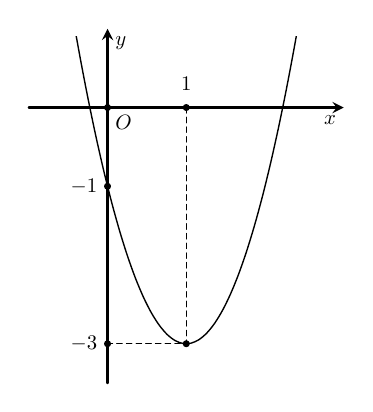
\begin{tikzpicture}[line join=round, line cap=round,>=stealth,thick,scale=1]
			\tikzset{every node/.style={scale=0.75}}
			\def\a{2} \def\b{-4} \def\c{-1} \def\rt{.03}
			\def\hf(#1){\a*(#1)^2+\b*(#1)+\c}
			\pgfmathsetmacro\tdx{-\b/(2*\a)} \pgfmathsetmacro\tdy{\hf(\tdx)}
			\def\xmin{\tdx-2} \def\xmax{\tdx+2}
			\def\ymin{\tdy-0.5} \def\ymax{\tdy+4}
			%\draw[color=gray!50,dashed] (\xmin,\ymin) grid (\xmax,\ymax);
			\draw[->] (\xmin,0)--(0,0) node[below right]{$O$}--(\xmax,0) node[below left] {$x$};
			\draw[->] (0,\ymin)--(0,\ymax) node[below right] {$y$};
			\draw[fill=black] (0,0) circle (\rt);
			\clip (\xmin+0.1,\ymin+0.1) rectangle (\xmax-0.1,\ymax-0.1);
			\draw[smooth,samples=100,line width=.5] plot(\x,{\hf(\x)});
			\foreach \y/\py in {-1/180}\draw[fill=black] (0,\y) circle (\rt)+(\py:.3) node{$\y$};
			\foreach \x/\y/\px/\py in {1/-3/90/180}{
				\draw[fill=black] (\x,0) circle (\rt)+(\px:.3) node{$\x$}
				(0,\y)circle (\rt)+(\py:.3) node{$\y$};
				\draw[fill=black] (\x,\y) circle (\rt);
				\draw[dash pattern=on 2pt off 1.5pt,thin] (\x,0)|-(0,\y);	}
	\end{tikzpicture}}
	\loigiai{
	Hàm số nghịch biến trên khoảng $(-\infty;1)$.
	}
\end{ex}
%%%Câu 8
\begin{ex}%[0H4N1-2]
	Cho $\alpha$ là góc tù. Điều khẳng định nào sau đây là \textbf{sai}?
	\choice
	{$\sin \alpha >0$}
	{$\cos \alpha <0$}
	{$\tan \alpha <0$}
	{\True $\cot \alpha >0$}
	\loigiai{
		Do $\alpha$ là góc tù, suy ra $\cos \alpha<0;\ \sin \alpha>0$. Nên $\tan \alpha<0$, $\cot \alpha<0$. Nên $\cot \alpha>0$ sai.}
\end{ex}
%%%Câu 9
\begin{ex}%[0D4H2-1]
	Cho tam giác $ABC$ có $AB=4$, $BC=7$, $AC=9$. Tính $\sin A$.
	\choice
	{$\sin A=\dfrac{\sqrt{3}}{3}$}
	{$\sin A=-\dfrac{\sqrt{5}}{3}$}
	{$\sin A=\pm \dfrac{\sqrt{5}}{3}$}
	{\True $\sin A=\dfrac{\sqrt{5}}{3}$}
	\loigiai{
		Áp dụng định lí côsin cho $\triangle ABC$, ta có $BC^2=AB^2+AC^2-2AB\cdot AC\cdot\cos A$.\\
		Suy ra $\cos A=\dfrac{AB^2+AC^2-BC^2}{2\cdot AB\cdot AC}=\dfrac{4^2+9^2-7^2}{2\cdot 4\cdot 9}=\dfrac{2}{3}$.\\
		Ta có $\sin^2 A+\cos^2 A=1\Leftrightarrow \sin^2 A=1-\cos^2 A=1-\left(\dfrac{2}{3}\right)^2=\dfrac{5}{9}\Rightarrow \sin A=\dfrac{\sqrt{5}}{3}$.\\
		Vậy $\sin A=\dfrac{\sqrt{5}}{3}$.}
\end{ex}
%%%Câu 10
\begin{ex}%[0D4H2-1]
	Cho tam giác $ABC$ cân tại $A$ có cạnh $b=30$ và $A=120^\circ$. Bán kính đường tròn ngoại tiếp của tam giác $ABC$ là
	\choice
	{$R=30\sqrt{3}$}
	{$R=15\sqrt{3}$}
	{\True $R=30$}
	{$R=30\sqrt{2}$}
	\loigiai{
		Áp dụng định lí Côsin cho tam giác $ABC$, ta có
		\[a^2=b^2+c^2-2bc\cdot \cos A=30^2+30^2-2\cdot 30\cdot 30\cdot \cos{120^\circ}=2\,700.\]
		Suy ra $a=30\sqrt{3}$.
		Áp dụng định lí sin cho tam giác $ABC$, ta có
		$R=\dfrac{a}{2\sin A}=\dfrac{30\sqrt{3}}{2\sin{120^\circ}}=30$.\\
		Vậy bán kính đường tròn ngoại tiếp tam giác $ABC$ là $R=30$.}
\end{ex}
%%%Câu 11
\begin{ex}%[0D1H3-1]
	Cho hai tập hợp $A=\{x\in\mathbb{Z}\mid-2<x\le 4\}$, $B=\{x\in\mathbb{Z}\mid |x|\le 2\}$. Tìm $A\cap B$.
	\choice
	{$A\cap B=\{-1;0;2;3\}$}
	{\True $A\cap B=\{-1;0;1;2\}$}
	{$A\cap B=\{-2;0;1;2\}$}
	{$A\cap B=\{-2;-1;1;2\}$}
	\loigiai{
		Ta có $A=\{x\in\mathbb{Z}\mid-2<x\le 4\}\Rightarrow A=\{-1;0;1;2;3;4\}$.\\
		$B=\{x\in\mathbb{Z}\mid|x|\le 2\}\Rightarrow B=\{-2;-1;0;1;2\}$.\\
		Vậy $A\cap B=\{-1;0;1;2\}$.
	}
\end{ex}
%%%Câu 12
\begin{ex}%[0D4V3-1]
	Hai chiếc tàu thủy $P$ và $Q$ trên biển cách nhau $100$ m và thẳng hàng với chân $A$ của tháp hải đăng $AB$ trên bờ biển. Từ $P$ và $Q$ người ta nhìn chiều cao $AB$ của tháp dưới các góc $\widehat{BPA}=15^\circ$ và $\widehat{BQA}=55^\circ$. Tính chiều cao của tháp (kết quả làm tròn đến hàng đơn vị).
	\choice
	{$30$}
	{$32$}
	{$34$}
	{\True $33$}
	\loigiai{
		\immini{
			Ta có $\widehat{PBQ}=55^\circ-15^\circ=40^\circ$.\\
			Áp dụng định lý $\sin$ cho tam giác $PBQ$ ta có $\dfrac{BQ}{\sin 15^\circ}=\dfrac{100}{\sin 40^\circ}\Leftrightarrow BQ=\dfrac{100\cdot\sin 15^\circ}{\sin 40^\circ}$.\\
			Khi đó, chiều cao của tháp là $AB=\sin 55^\circ\cdot BQ\approx 33$ m.	
		}
		{
			\begin{tikzpicture}[scale=1, font=\footnotesize, line join=round, line cap=round, >=stealth]
				\path
				(0,0) coordinate (P)++(0:5)coordinate(Q)++(0:1.15)coordinate(A)++(90:1.65)coordinate(B)
				;
				\draw (P)--(Q)node[midway,above]{$100$ m}--(A)--(B)--cycle
				(B)--(Q)
				;
				\foreach \x/\g in {A/-90,B/90,P/-90,Q/-90}\fill[black] (\x) circle (1pt)+(\g:.3)node{$\x$};
				\draw pic[draw, angle radius = 12pt, "$15^\circ$", angle eccentricity = 1.5]{ angle = A--P--B};
				\draw pic[draw, angle radius = 12pt, "$55^\circ$", angle eccentricity = 1.5]{ angle = A--Q--B};
			\end{tikzpicture}
		}
	}
\end{ex}
\Closesolutionfile{ans}
\indapan{6}{ans/ans-CTST-0-OTGK1-De05-LC}
%-------------------------------------------
\cauds
\Opensolutionfile{ans}[ans/ans-CTST-0-OTGK1-De05-DS]
%%%Câu 1
\begin{ex}%[0D1H3-2]
	Cho hai tập hợp $A=\{0;1;2;3;4\}$, $B=\{3;4;5;6\}$. Khi đó
	\choiceTF
	{\True $A\cup B=\{0;1;2;3;4;5;6\}$}
	{$A\cap B=\{5;6\}$}
	{$B\setminus A=\{0;1;2\}$}
	{\True $(A\cup B)\setminus (A\cap B)=(A\setminus B)\cup (B\setminus A)$}
	\loigiai{
		\begin{itemchoice}
			\itemch \textbf{Đúng}. $A\cup B=\{0;1;2;3;4;5;6\}$.
			\itemch \textbf{Sai}. $A\cap B=\{3;4\}$.
			\itemch \textbf{Sai}. Ta có $B\setminus A=\{5;6\}$.
			\itemch \textbf{Đúng}. $A\cup B=\{0;1;2;3;4;5;6\}$, $A\cap B=\{3;4\}$ nên $(A\cup B)\setminus (A\cap B)=\{0;1;2;5;6\}$;
			$A\setminus B=\{0;1;2\}$, $B\setminus A=\{5;6\}$ nên $(A\setminus B)\cup (B\setminus A)=\{0;1;2;5;6\}$.
		\end{itemchoice}
	}
\end{ex}
%%%Câu 2
\begin{ex}%[0D3H1-5]
	Cho hệ bất phương trình $\heva{&x+2y-100\le 0\\&2x+y-80\le 0\\&x\ge 0\\&y\ge 0}$.Khi đó
	\choiceTF
	{Hệ trên không phải là một hệ bất phương trình bậc nhất hai ẩn}
	{$(-1;2)$ là một nghiệm của hệ bất phương trình trên}
	{\True $(-1;5)$ không là một nghiệm của hệ bất phương trình trên}
	{\True Miền nghiệm của hệ bất phương trình trên là một miền tứ giác}
	\loigiai{
		\begin{itemchoice}
			\itemch \textbf{Sai}. Hệ trên là một hệ bất phương trình bậc nhất hai ẩn.
			\itemch \textbf{Sai}. Thay $x=-1$; $y=2$  vào hệ bất phương trình ta được $\heva{&-97\le 0\\&-80\le 0\\&-1\ge 0\\&2\ge 0}$  (Vô lý).\\ Vậy $(-1;2)$ không phải là một nghiệm của hệ bất phương trình.
			\itemch \textbf{Đúng}. Thay $x=-1$; $y=5$ vào hệ bất phương trình ta được $\heva{&-91\le 0\\&-77\le 0\\&-1\ge 0\\&5\ge 0}$ (Vô lý).\\ Vậy $(-1; 5)$ không là một nghiệm của hệ bất phương trình.
			\itemch \textbf{Đúng}. Vẽ đường thẳng $d_1\colon x+2y-100=0$. Vì $0+2\cdot 0-100\le 0$ nên toạ độ điểm $O(0;0)$ thoả mãn bất phương trình $x+2y-100\le 0$. Do đó miền nghiệm $D_1$ của bất phương trình $x+2y-100\le 0$ là nửa mặt phẳng bờ $d_1\colon x+2y-100=0$ chứa gốc toạ độ $O$.\\ 
			Tương tự miền nghiệm $D_2$ của bất phương trình $2x+y-80\le 0$ là nửa mặt phẳng bờ $d_2\colon 2x+y-80=0$ chứa gốc toạ độ $O$.\\  
			Tương tự miền nghiệm $D_3$ của bất phương trình $x\ge 0$ là nửa mặt phẳng bờ $Oy$ chứa điểm $(1;0)$.\\
			Tương tự miền nghiệm $D_3$ của bất phương trình $y\ge 0$ là nửa mặt phẳng bờ $Ox$ chứa điểm $(0;1)$.\\
			Khi đó miền nghiệm của hệ bất phương trình là miền tứ giác $OABC$.
			\begin{center}
				\begin{tikzpicture}[scale=0.6,thick,>=stealth']
					\draw[->] (-3,0) -- (12,0)node[above]{$x$};
					\draw[->,color=black] (0,-2) -- (0,9)node[right]{$y$};
					\node[below left] at (0,0) {$O$};
					\clip(-3,-2) rectangle (12,9);
					\draw[line width=1.2pt,smooth,samples=100,domain=-1:9] plot(\x,{-2*(\x)+8});
					\draw[line width=1.2pt,smooth,samples=100,domain=-1:15.3] plot(\x,{-0.5*(\x)+5});
					\fill[pattern=north east lines] (0,0)--(0,5) --(2,4)--(4,0)-- cycle;
					\node[above] at (4,0) {$A$};
					\node[below] at (4,0) {$40$};\node[below] at (10,0) {$100$};
					\node[right] at (0,5) {$B$}; \node[left] at (0,5) {$50$};
					\node[left] at (0,8) {$80$};
					\node[right] at (2,4) {$C$};\node[left] at (0,4) {$40$};
					\node[below] at (2,0) {$20$};\draw[dashed] (0,4)--(2,4)--(2,0);
				\end{tikzpicture}
			\end{center}
		\end{itemchoice}
	}
\end{ex}
%%%Câu 3
\begin{ex}%[0D3H1-3]
	Cho hàm số $y=f(x)=\dfrac{\sqrt{4-x}}{x-2}$.
	\choiceTF
	{$f(-5)=\dfrac{3}{7}$}
	{\True Điểm $M(3;1)$ thuộc đồ thị hàm số $y=f(x)$}
	{\True Đồ thị hàm số $y=f(x)$ cắt trục $Oy$ tại điểm $A(0;-1)$}
	{Có $5$ số tự nhiên thuộc tập xác định của hàm số $y=f(x)$}
	\loigiai{
		\begin{itemchoice}
			\itemch Sai. Vì $f(-5)=\dfrac{\sqrt{4-(-5)}}{(-5)-2}=-\dfrac{3}{7}$.
			\itemch Đúng. Vì $f(3)=\dfrac{\sqrt{4-3}}{3-2}=1 \Rightarrow M(3;1)$ thuộc đồ thị hàm số $y=f(x)$.
			\itemch Đúng. Vì $f(0)=\dfrac{\sqrt{4-0}}{0-2}=-1$ nên đồ thị hàm số $y=f(x)$ cắt trục $Oy$ tại điểm $A(0;-1)$.
			\itemch Sai. Điều kiện:			
			$\heva{&4-x\ge 0\\&x-2\ne 0}
			\Leftrightarrow \heva{&x \le 4\\&x \ne 2.}$ \\
			$\Rightarrow$ tập hợp các số tự nhiên thuộc tập xác định của hàm số đã cho là $\{0;1;3;4\}$.\\
			Do đó, có $4$ số tự nhiên thuộc tập xác định của hàm số đã cho nên mệnh đề sai.
		\end{itemchoice}
	}
\end{ex}
%%%Câu 4
\begin{ex}%[0H4H2-2]
	Cho tam giác $ABC$ có $BC=a$, $AC=b$, $AB=c$ và $b=8$, $c=5$, $A=60^\circ$.
	\choiceTF
	{\True Độ dài cạnh $a=7$}
	{ Diện tích của tam giác $ABC$ bằng $10$}
	{\True Bán kính đường tròn ngoại tiếp tam giác $AC$ bằng $\dfrac{7 \sqrt{3}}{3}$}
	{ Bán kính đường tròn nội tiếp tam giác $ABC$ bằng $\dfrac{\sqrt{3}}{2}$}
	\loigiai{
		\begin{itemchoice}
			\itemch Ta có $$a=\sqrt{b^2+c^2-2bc\cdot \cos A}=\sqrt{8^{2}+5^{2}-2\cdot 8\cdot 5\cdot \cos 60^\circ}=7.$$
			\itemch Diện tích của tam giác $ABC$ là $$S=\dfrac{1}{2} b\cdot c\cdot \sin A=\dfrac{1}{2} \cdot 8 \cdot 5 \cdot \sin 60^{\circ}=10 \sqrt{3}.$$
			\itemch  Bán kính đường tròn ngoại tiếp tam giác $A B C$ là $$R=\dfrac{a\cdot b\cdot  c}{4 S}=\dfrac{7\cdot 8 \cdot 5}{4\cdot 10\sqrt{3}}=\dfrac{7\sqrt{3}}{3}.$$
			\itemch  Bán kính đường tròn nội tiếp tam giác $ABC$ là $$r=\dfrac{2 S}{a+b+c}=\dfrac{2\cdot 10\sqrt{3}}{7+8+5}=\sqrt{3}.$$
	\end{itemchoice}}
\end{ex}
\Closesolutionfile{ans}
\indapan{2}{ans/ans-CTST-0-OTGK1-De05-DS}
\caukq
\Opensolutionfile{ans}[ans/ans-CTST-0-OTGK1-De05-KQ]
%%%Câu 1
\begin{ex}%[0D2H2-2] 
	Cho $\tan \alpha -\cot \alpha =3$. Tính giá trị  biểu thức  $A=\tan^2 \alpha +\cot^2 \alpha$.
	 \shortans{$11$}
	\loigiai{
		 $A={\tan }^2\alpha +{\cot }^2\alpha \Leftrightarrow A=\left( \tan \alpha -\cot \alpha \right)^2+2\tan \alpha .\cot \alpha \Leftrightarrow A=3^2+2\Leftrightarrow A=11$.
	}
\end{ex}
%%%Câu 2
\begin{ex}%[0D2H2-2] 
	Tìm giá trị lớn nhất của biểu thức $F(x;y)=x+2y$, biết $x$, $y$ thỏa mãn các điều kiện $\heva{&0\le y\le 4\\& x\ge 0\\& x-y-1\le 0\\& x+2 y-10\le 0.}$	
	\shortans{$3228$}
	\loigiai{
		Vẽ đường thẳng $d_1\colon x-y-1=0$, đường thẳng $d_1$ qua hai điểm $(0 ;-1)$ và $(1;0)$.\\
		Vẽ đường thẳng $d_2\colon x+2y-10=0$, đường thẳng $d_2$ qua hai điểm $(0 ;5)$ và $(2;4)$.\\
		Vẽ đường thẳng $d_3\colon y=4$.
		\begin{center}
			\begin{tikzpicture}[>=stealth,x=1cm,y=1cm,scale=1]
				\draw[->] (-2,0)--(7,0)node[below right]{$x$};
				\draw[->] (0,-2)--(0,7) node[left]{$y$};
				\draw (0,0)node[above right]{$O$};
				\path[pattern=horizontal lines] (-1,-2)-|(7,6)--cycle;
				\draw (-1,-2)node[below left]{$d_1$}--(7,6);
				\path[pattern=crosshatch dots] (-2,6)|-(7,7)--(7,1.5)--cycle;
				\draw (-2,6)node[below left]{$d_2$}--(7,1.5);
				\path[pattern=vertical lines] (-2,7)rectangle(7,4);
				\draw (-2,4)node[below left]{$d_3$}--(7,4);
				\path[pattern=crosshatch] (-2,-2)rectangle(7,0);
				\draw (-2,0)--(7,0);
				\path[pattern=north east lines] (-2,-2)rectangle(0,7);
				\draw (0,-2)--(0,7);
				\draw[dashed] (4,0)--(4,3)node[above left]{$A$}--(0,3) circle (1pt);
				\draw[dashed] (2,0)--(2,4)node[below left]{$B$}--(0,4)node[below right]{$C$} circle (1pt);
				\draw (1,0)node[above]{$E$} circle (1pt);
			\end{tikzpicture}
		\end{center}
		Miền nghiệm là ngũ giác $ABCOE$ với $A(4;3)$, $B(2;4)$, $C(0;4)$, $E(1;0)$.\\
		Ta có $F(4;3)=10$, $F(2;4)=10$, $F(0;4)=8$, $F(1;0)=1$, $F(0;0)=0$.\\
		Vậy giá trị lớn nhất của biết thức $F(x;y)=x+2y = 10$.	
	}
\end{ex}
%%%Câu 3
\begin{ex}%[0D2V2-2] 
	Trong một dây chuyền sản xuất có hai công nhân là An và Bình. Dây chuyền này sản xuất ra sản phẩm loại $I$ và loại $II$. Mỗi sản phẩm loại $I$, loại $II$ bán ra thu về lợi nhuận lần lượt là $35\,000$ đồng và $50\,000$ đồng. Để sản xuất được sản phẩm loại $I$ thì An phải làm việc trong $1$ giờ, Bình phải làm việc trong $30$ phút. Để sản xuất được sản phẩm loại $II$ thì An phài làm việc trong $30$ phút, Bình phải làm việc trong $45$ phút. Một người không thể làm đồng thời hai loại sản phẩm. Biết rằng trong một ngày An không thể làm việc quá $12$ giờ, Bình không thể làm việc quá $10$ giờ. Tìm lợi nhuận lớn nhất trong một ngày của dây chuyền sản xuất (đơn vị tính: nghìn đồng).	\shortans{$680$}
	\loigiai{
		Gọi $x$, $y$ lần lượt là số sản phẩm loại $I$ và loại $II$ được sản xuất $(x \in \mathbb{N}$, $y \in \mathbb{N})$.\\
		Ta có hệ bất phương trình sau $\heva{&x+0{,}5 y\le 12\\& 0{,}5 x+0{,}75 y \le 10\\& x \ge 0\\& y\ge 0.}\quad(*)$\\
		Miền nghiệm của hệ bất phương trình $(*)$ được biểu diễn là	
		\begin{center}
			\begin{tikzpicture}[>=stealth,x=1cm,y=1cm,scale=.35]
				\draw[->] (-2,0)--(20,0)node[below right]{$x$};
				\draw[->] (0,-2)--(0,25) node[left]{$y$};
				\path[pattern=crosshatch dots] (-0.5,25)-|(20,-2)--(13,-2)--cycle;
				\draw (-0.5,25)--(13,-2);
				\path[pattern=grid] (-2,14.67)|-(20,25)--(20,0)--cycle;
				\draw (-2,14.67)--(20,0);
				\path[pattern=north west lines] (-2,-2)rectangle(0,25);
				\draw (0,-2)--(0,25);
				\path[pattern=north west lines] (-2,-2)rectangle(20,0);
				\draw (-2,0)--(20,0);
				\draw (0,0)node[above right]{$O$};
				\draw (0,13.33)node[below right]{$A$};
				\draw (8,8)node[left]{$B$};
				\draw (12,0)node[above left]{$12$};
				\draw (12,0)node[above right]{$C$};
				\draw[dashed](8,0)node[above left]{$8$}--(8,8)--(0,8)node[above right]{$8$};	
			\end{tikzpicture}
		\end{center}
		Lợi nhuận trong một ngày của dây chuyển sản xuất là $T=35\,000x+50\,000 y$ (đồng).\\
		Dựa vào miền nghiệm, ta thấy $T$ chi đạt giá trị lớn nhất tại các điểm $O$, $A$, $B$, $C$.\\
		Mà $A$ có tọa độ không nguyên nên loại.\\
		Tại $O(0;0)\Rightarrow T=0$ đồng.\\
		Tại $B(8;8)\Rightarrow T=35\,000\cdot 8+50\,000\cdot 8=680\,000$ đồng.\\
		Tại $C(12;0) \Rightarrow T=35\,000\cdot 12+50\,000=420\,000$ đồng.\\
		Vậy lợi nhuận lớn nhất trong ngày là $680\,000$ đồng.
	}
\end{ex}
%%%Câu 4
\begin{ex}%[0D3V1-7]
	Một hãng xe taxi niêm yết giá cước khi đi xe theo bảng sau:
	\begin{center}
		\begin{tabular}{|l|c|c|c|}
			\hline & Dưới $60$ km & $60-180$ km & Trên $180$ km \\
			\hline \begin{tabular}{l} 
				Xe $4$ chỗ \\
				(Vios, Honda City, \\
				Mazda3, i10)
			\end{tabular} & $11000$ đồng/km & $10000$ đồng/km & $9000$ đồng/km \\
			\hline \begin{tabular}{l} 
				Xe $7$ chỗ \\
				(Innova, Fortuner, \\
				Sorento)
			\end{tabular} & $13000$ đồng/km & $12000$ đồng/km & $11000$ đồng/km \\
			\hline Thời gian chờ & \multicolumn{3}{|c|}{$30000$ đồng/giờ } \\
			\hline
		\end{tabular}
	\end{center}
	Tính số tiền phải trả (tính theo đơn vị nghìn đồng) khi đi xe taxi $7$ chỗ một quãng đường là $265$ km, biết rằng giữa đường đi xe cần dừng lại $1$ giờ để ăn trưa.
	\shortans{$3228$}
	\loigiai{
		Gọi $x$ là số km thực đi của xe taxi và $y$ (nghìn đồng) là số tiền phải trả (không tính số tiền trả cho thời gian chờ đợi).\\
		Ta có hàm số:
		$y=f(x)=\heva{&13x &\text{khi} && 0\le x<60\\&59\cdot 13+(x-59)\cdot 12 &\text{khi} && 60\le x\le 180\\&59\cdot 13+121\cdot 12+(x-180)11\,000 &\text{khi} &&x>180.}$\\
		Khi $x=265$ thì $y=f(265)=59\cdot 13+121\cdot 12+(269-180)\cdot 11=3\,198$ nghìn đồng.\\
		Vậy tổng số tiền người đi xe phải trả là $3198+30=3\,228$ nghìn đồng.}
\end{ex}
%%%Câu 5
\begin{ex}%[0H2B3-4]
	Hai chiếc tàu thuỷ cùng xuất phát từ vị trí $A$, đi thẳng theo hai hướng tạo với nhau một góc $60^\circ$. Tàu thứ nhất chạy với tốc độ $30$ km/h, tàu thứ hai chạy với tốc độ $38$ km/h. Hỏi sau $2$ giờ hai tàu cách nhau bao nhiêu km? \shortans{$69{,}4$}
	\loigiai{
		\immini{
			Gọi $B$, $C$ lần lượt là vị trí của tàu $1$ và tàu $2$ đi được sau $2$ giờ. \\
			Dễ thấy $AB =2\cdot 30= 60$ km; $AC =2\cdot 38=76$ km.\\
			Áp dụng định lí cô sin cho tam giác $ABC$, ta có \\
			$BC^2 = AB^2 + AC^2 - 2AB\cdot AC \cdot \cos A = 4816$ \\$\Rightarrow  BC = 4\sqrt{301} \approx 69{,}4$ km.\\
			Vậy khoảng cách giữa hai tàu là $69{,}4$ km.
		}
		{
			\begin{tikzpicture}[scale=.7, font=\footnotesize, line join=round, line cap=round,>=stealth]
				\path
				(0,0) coordinate (A)
				(3.5,0) coordinate (B)
				;
				\coordinate (C) at ($(A)+(60:4)$) ; 
				\draw (A)--(B)--(C)--(A) 
				pic["$60^{\circ}$", draw=black, angle eccentricity=1.5, angle radius=0.7cm]{angle=B--A--C};
				\foreach \x/\g in {A/-120,B/-60,C/90} 
				\fill[black] (\x) circle (1pt)+(\g:3mm) node {$\x$};
			\end{tikzpicture}
		}
	}
\end{ex}
%%%Câu 6
\begin{ex}%[0H2B3-4]
	\immini[thm]{
		Từ đỉnh của một tòa nhà người ta đo được góc tạo bởi hướng nhìn đến đỉnh của tháp truyền thông và phương ngang là $15^\circ$. Từ chân  tòa nhà đó  người ta đo được góc tạo bởi hướng nhìn đến đỉnh của tháp truyền thông và phương ngang là $29^\circ$. Biết tòa nhà cao $50$ m, tính chiều cao của tháp (đơn vị m).
			\shortans{$96{,}8$}
	}
	{
		\begin{tikzpicture}[scale=1, font=\footnotesize, line join=round, line cap=round,>=stealth]
			\path 
			(0,4.5) coordinate (A)
			(0,-1) coordinate (H)
			(4,3) coordinate (B)
			(4,-1) coordinate (C) 
			(0,3) coordinate (K) 
			;
			\draw [fill=gray!60]
			(-0.4,-1)
			.. controls ++(50:0.5) and ++(265: 1) .. (0,4.5) 
			.. controls ++(-85:1) and ++(130: 0.5) .. (0.4,-1)--cycle;
			\draw[pattern=bricks,pattern color=brown] (B)--(6,3)--(6,-1)--(4,-1)--(B);
			\foreach \i in {2,3,4,5}
			\draw[fill=white] ({4+1/3},{-1+(2/3)*(\i-1)})--({4+1/3},{-1+(2/3)*(\i-1)+0.5})--({4+2/3},{-1+(2/3)*(\i-1)+0.5})--({4+2/3},{-1+(2/3)*(\i-1)})--cycle 
			({5+1/3},{-1+(2/3)*(\i-1)})--({5+1/3},{-1+(2/3)*(\i-1)+0.5})--({5+2/3},{-1+(2/3)*(\i-1)+0.5})--({5+2/3},{-1+(2/3)*(\i-1)})--cycle;
			\draw[dashed](A)--(B)--(K)  (A)--(C); 
			\draw pic["$29^{\circ}$", draw=black, angle eccentricity=1.4, angle radius=0.9cm]{angle=A--C--H};
			\draw pic["$15^{\circ}$", draw=black,double, angle eccentricity=1.5, angle radius=1.2cm]{angle=A--B--K};
			\foreach \x/\g in {A/180,B/90,C/140} 
			\fill[black] (\x) circle (1pt)+(\g:3mm) node {$\x$};
			\clip (-0.7,{-1-0.25}) rectangle (6.6,-1) ;
			\draw[fill=gray!30] (-0.7,-1)--(6.6,-1)--(6.6,{-1-0.25})--(-0.7,{-1-0.25})--cycle;
			\foreach \i in {1,2,...,35}
			\draw ({-0.5+0.2*(\i)},-1)--($({-0.5+0.2*(\i)},-1)+(-120:0.3)$) ;
		\end{tikzpicture}
	}
	\loigiai{
		\begin{center}
			\begin{tikzpicture}[scale=1, font=\footnotesize, line join=round, line cap=round,>=stealth]
				\path 
				(0,4.5) coordinate (A)
				(0,-1) coordinate (H)
				(4,3) coordinate (B)
				(4,-1) coordinate (C) 
				(0,3) coordinate (K) 
				;
				\draw [fill=gray!60]
				(-0.4,-1)
				.. controls ++(50:0.5) and ++(265: 1) .. (0,4.5) 
				.. controls ++(-85:1) and ++(130: 0.5) .. (0.4,-1)--cycle;
				\draw[pattern=bricks,pattern color=brown] (B)--(6,3)--(6,-1)--(4,-1)--(B);
				\foreach \i in {2,3,4,5}
				\draw[fill=white] ({4+1/3},{-1+(2/3)*(\i-1)})--({4+1/3},{-1+(2/3)*(\i-1)+0.5})--({4+2/3},{-1+(2/3)*(\i-1)+0.5})--({4+2/3},{-1+(2/3)*(\i-1)})--cycle 
				({5+1/3},{-1+(2/3)*(\i-1)})--({5+1/3},{-1+(2/3)*(\i-1)+0.5})--({5+2/3},{-1+(2/3)*(\i-1)+0.5})--({5+2/3},{-1+(2/3)*(\i-1)})--cycle;
				\draw[dashed](A)--(B)--(K)  (A)--(C) (A)--(H); 
				\draw pic["$29^{\circ}$", draw=black, angle eccentricity=1.4, angle radius=0.9cm]{angle=A--C--H};
				\draw pic["$15^{\circ}$", draw=black,double, angle eccentricity=1.5, angle radius=1.2cm]{angle=A--B--K};
				\foreach \x/\g in {A/180,B/90,C/140,K/180,H/140} 
				\fill[black] (\x) circle (1pt)+(\g:3mm) node {$\x$};
				\clip (-0.7,{-1-0.25}) rectangle (6.6,-1) ;
				\draw[fill=gray!30] (-0.7,-1)--(6.6,-1)--(6.6,{-1-0.25})--(-0.7,{-1-0.25})--cycle;
				\foreach \i in {1,2,...,35}
				\draw ({-0.5+0.2*(\i)},-1)--($({-0.5+0.2*(\i)},-1)+(-120:0.3)$) ;
			\end{tikzpicture}
		\end{center}
		Gọi $H$   là hình chiếu vuông góc của $A$ trên mặt đất,  $K$ là hình chiếu vuông góc của $B$ trên $AH$. \\
		Ta có $AH = CH\tan  \widehat{ACH} = CH \tan 29^\circ$, 
		$AK = BK\tan  \widehat{ABK} = CH \tan 15^\circ$. \\
		Khi đó 
		\begin{align*}
			&AH-AK = BC \\
			\Leftrightarrow ~ & CH \tan 29^\circ- CH \tan 15^\circ = 50\\
			\Leftrightarrow ~ & CH =  \dfrac{50}{ \tan 29^\circ- \tan 15^\circ}.
		\end{align*}
		Chiều cao của tháp là
		$$AH =CH\tan 29^\circ=\dfrac{50\tan 29^\circ}{\tan 29^\circ-\tan 15^\circ}\approx 96{,}8\mathrm{~m}.$$
	}
\end{ex}
\Closesolutionfile{ans}
\indapan{6}{ans/ans-CTST-0-OTGK1-De05-KQ}

